% Автоматически сгенерированный файл
\par\noindent Использован дополнительный модуль, написаный ИИ-моделью\par\vspace{4mm}
\par\noindent Использованные для измерения массы:\par\vspace{4mm}
\par
\begin{center}
\begin{tabular}{cccc}
\toprule
m0 & m1 & m2 & m3 \\
\midrule
1.095 & 1.4387 & 1.9333 & 2.8797 \\
\bottomrule
\end{tabular}
\end{center}

\par\noindent Теоретические частоты, расчитанные по формуле 9 лабораторной работы 
 для четных гармоник:\par\vspace{4mm}
\par
\begin{center}
\begin{tabular}{cccc}
\toprule
m0 & m1 & m2 & m3 \\
\midrule
274.9442 & 315.1538 & 365.3315 & 445.8729 \\
549.8884 & 630.3077 & 730.6629 & 891.7458 \\
824.8325 & 945.4615 & 1095.9944 & 1337.6187 \\
1099.7767 & 1260.6153 & 1461.3259 & 1783.4916 \\
1374.7209 & 1575.7691 & 1826.6574 & 2229.3646 \\
\bottomrule
\end{tabular}
\end{center}

\par\noindent Теоретические частоты, расчитанные по формуле 9 лабораторной работы 
 для нечетных гармоник:\par\vspace{4mm}
\par
\begin{center}
\begin{tabular}{cccc}
\toprule
m0 & m1 & m2 & m3 \\
\midrule
137.4721 & 157.5769 & 182.6657 & 222.9365 \\
412.4163 & 472.7307 & 547.9972 & 668.8094 \\
687.3604 & 787.8846 & 913.3287 & 1114.6823 \\
962.3046 & 1103.0384 & 1278.6602 & 1560.5552 \\
1237.2488 & 1418.1922 & 1643.9916 & 2006.4281 \\
\bottomrule
\end{tabular}
\end{center}

\par\noindent Измеренные частоты для нечетных гармоник:\par\vspace{4mm}
\par
\begin{center}
\begin{tabular}{cccc}
\toprule
m0 & m1 & m2 & m3 \\
\midrule
137.0 & 157.9 & 182.0 & 220.9 \\
413.8 & 475.5 & 544.4 & 666.3 \\
692.4 & 792.3 & 914.2 & 1107.1 \\
973.4 & 1113.3 & 1275.3 & 1550.0 \\
1260.2 & 1431.0 & 1643.1 & 2000.5 \\
\bottomrule
\end{tabular}
\end{center}

\par\noindent Измеренные частоты для четных гармоник:\par\vspace{4mm}
\par
\begin{center}
\begin{tabular}{cccc}
\toprule
m0 & m1 & m2 & m3 \\
\midrule
278.8 & 315.7 & 368.0 & 444.7 \\
559.6 & 634.4 & 733.8 & 888.0 \\
825.5 & 950.3 & 1093.0 & 1347.0 \\
1101.4 & 1263.7 & 1459.0 & 1790.1 \\
1366.6 & 1564.1 & 1833.8 & 2246.9 \\
\bottomrule
\end{tabular}
\end{center}

\par
\begin{figure}[H]
    \centering
    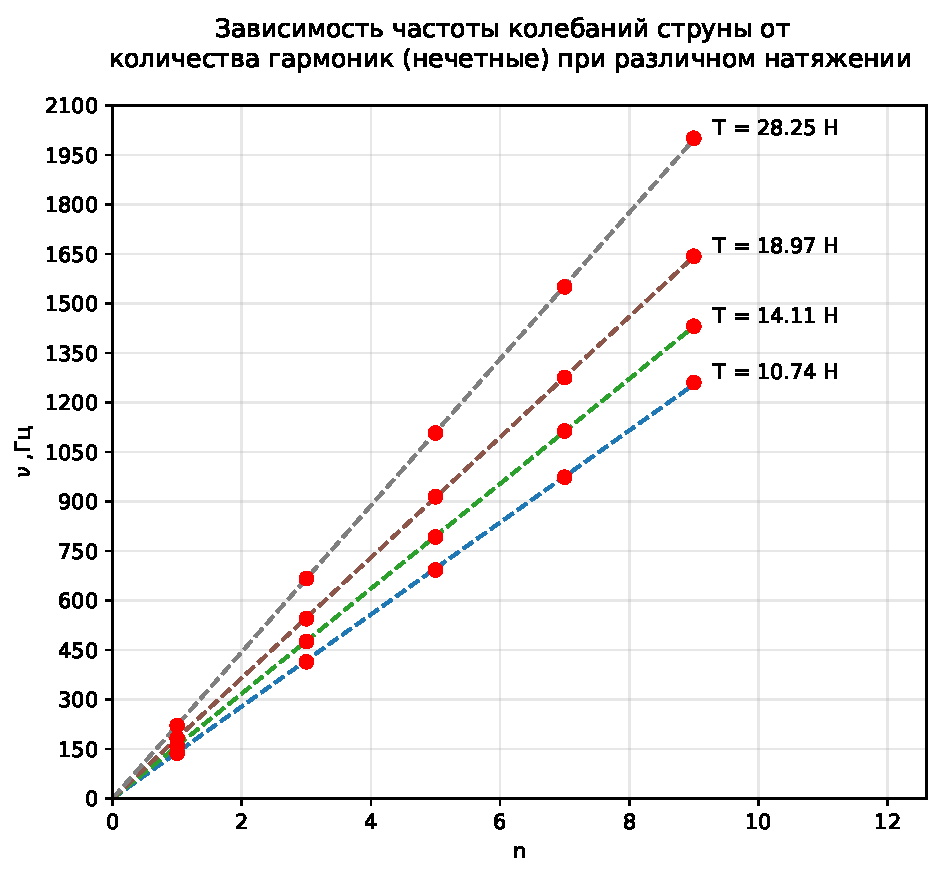
\includegraphics[width=0.7\textwidth]{export/uneven_plot.pdf}
    \caption{}
    \label{}
\end{figure}

\par
\begin{figure}[H]
    \centering
    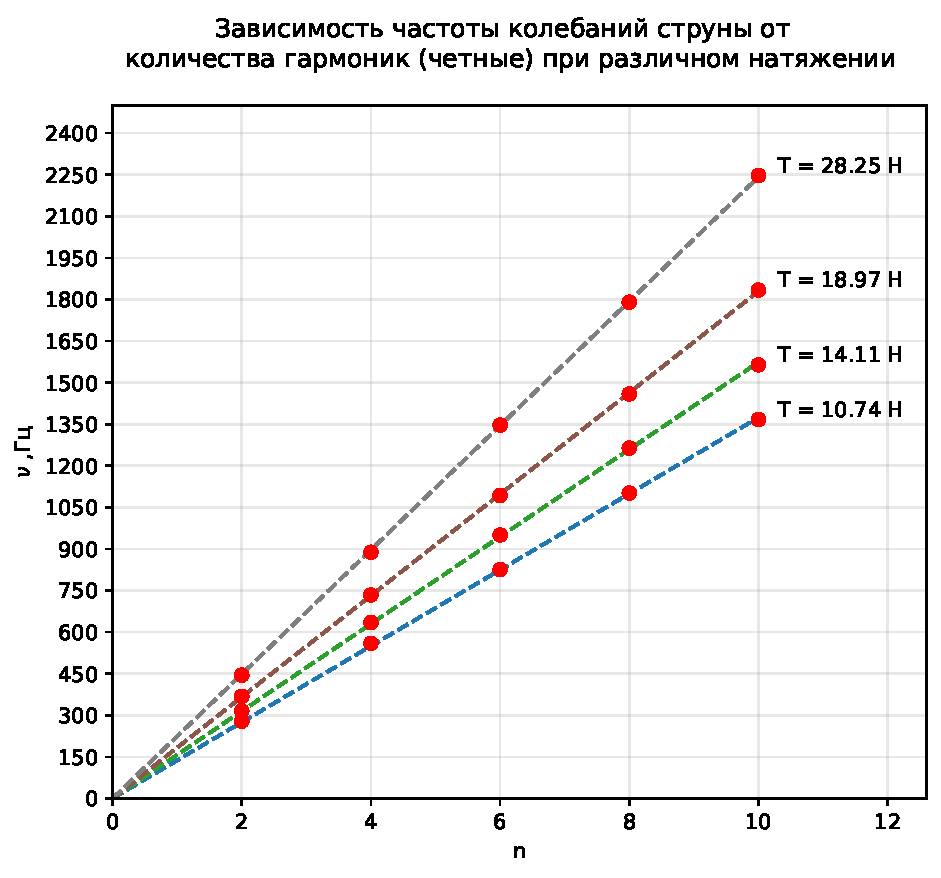
\includegraphics[width=0.7\textwidth]{export/even_plot.pdf}
    \caption{}
    \label{}
\end{figure}

\par\noindent Формулы для расчёта скорости волны из полученнного коэффициента наклона:\par\vspace{4mm}
\[\displaystyle k = \frac{\sqrt{\frac{T}{\rho}}}{2 L}\]\vspace{4mm}
\[\displaystyle u = 2 L k\]\vspace{4mm}

\par\noindent Формулы скорости волны (м/с), полученные из коэффициента наклона графика (МНК):\par\vspace{4mm}
\par\noindent Для нечетных гармоник:\par\vspace{4mm}
\par
\begin{center}
\begin{tabular}{ccccc}
\toprule
  & m0 & m1 & m2 & m3 \\
\midrule
$u_{prac}$ & 139.37 & 158.9 & 182.43 & 221.88 \\
$u_{teor}$ & 137.47 & 157.58 & 182.67 & 222.94 \\
$u_{error, \%}$ & 1.38 & 0.84 & 0.13 & 0.47 \\
\bottomrule
\end{tabular}
\end{center}

\par\noindent Для четных гармоник:\par\vspace{4mm}
\par
\begin{center}
\begin{tabular}{ccccc}
\toprule
  & m0 & m1 & m2 & m3 \\
\midrule
$u_{prac}$ & 137.39 & 157.37 & 182.91 & 224.15 \\
$u_{teor}$ & 137.47 & 157.58 & 182.67 & 222.94 \\
$u_{error, \%}$ & 0.06 & 0.13 & 0.13 & 0.54 \\
\bottomrule
\end{tabular}
\end{center}

\par\noindent где,\par\vspace{4mm}
\par\noindent $u_{teor}$ - скорость, расчитанная по формуле (2) лаб. работы\par\vspace{4mm}
\par\noindent $u_{prac}$ - скорость, расчитанная по коэффициенту наклона (2) лаб. работы\par\vspace{4mm}
\par\noindent $u_{error}$ - относительная ошибка практического измерения\par\vspace{4mm}
\par\noindent Расчет погонной плотности:\par\vspace{4mm}
\par
\begin{figure}[H]
    \centering
    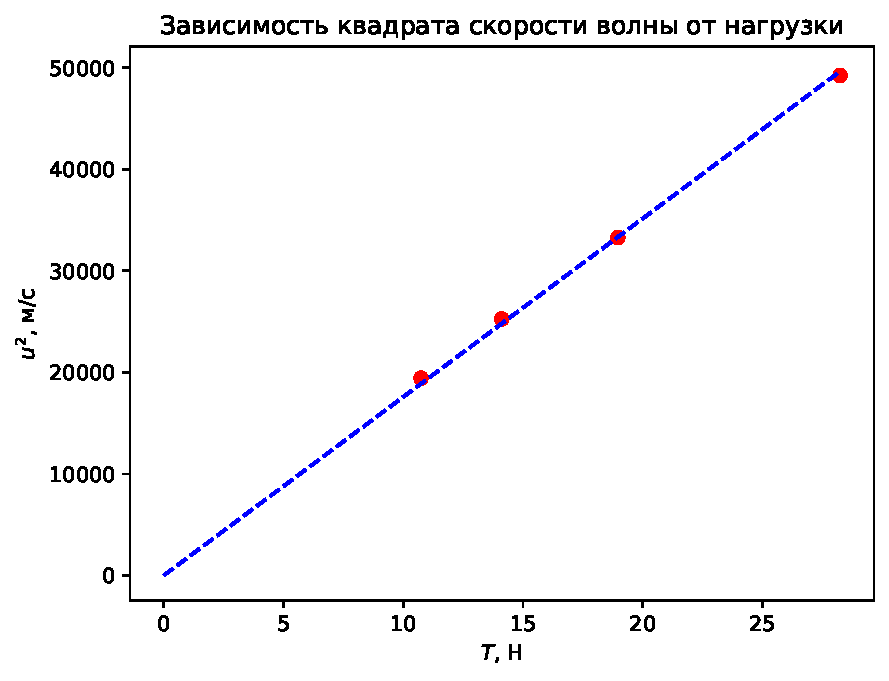
\includegraphics[width=0.7\textwidth]{export/u2_uneven.pdf}
    \caption{}
    \label{}
\end{figure}

\par
\begin{figure}[H]
    \centering
    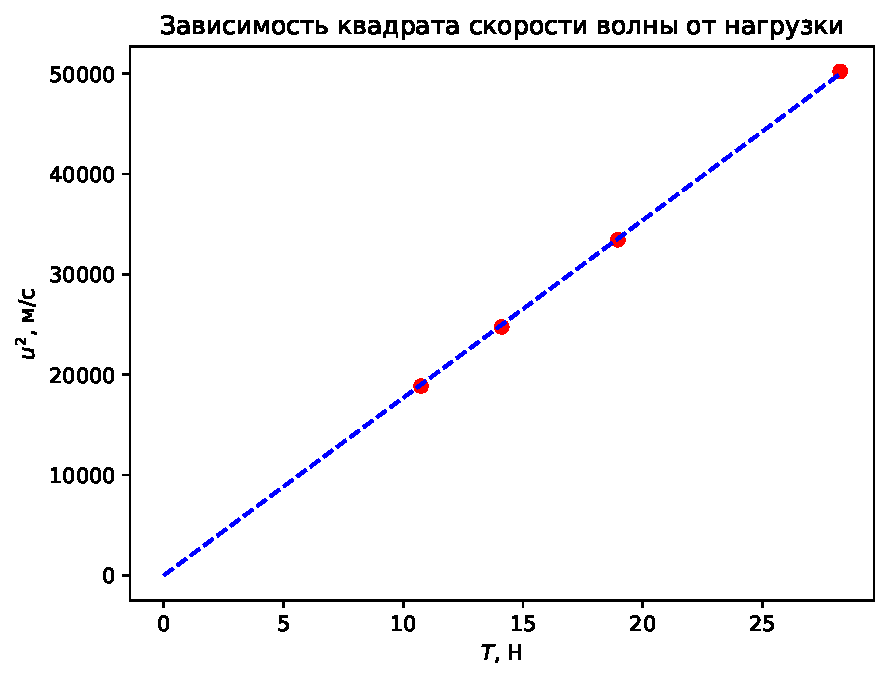
\includegraphics[width=0.7\textwidth]{export/u2_even.pdf}
    \caption{}
    \label{}
\end{figure}

\par\noindent Расчитанный из коэффициента наклона $\rho$ :\par\vspace{4mm}
\par\noindent $\rho_1 = 569,14 \times 10^{-6}$\par\vspace{4mm}
\par\noindent $\rho_1 = 564,94 \times 10^{-6}$\par\vspace{4mm}
\par\noindent $\rho_{error} = 0.6 \%$\par\vspace{4mm}
\par\noindent Вывод: все экспериментально рассчитанные значения лежат в пределах 5% 
 погрешности относительно теоретических. 
 Измерения частот проведены достаточно точно.\par\vspace{4mm}
